\documentclass[10pt]{article}
\usepackage{NotesTeXV3}

\usepackage{color}
\usepackage[dvipsnames]{xcolor}
\definecolor{myblue}{rgb}{0.10,0.11,0.8}
\definecolor{myred}{rgb}{0.74,0.1,0.05}
\definecolor{mygreen}{rgb}{0.,0.52,0.32}
\definecolor{myyellow}{rgb}{0.96,0.92,0.13}
\definecolor{myorange}{rgb}{0.7,0.41,0.1}
\definecolor{mypurple}{rgb}{0.51,0.02,.8}
\definecolor{mygray}{rgb}{0.6,0.6,0.6}
\renewcommand\emph[2][myred]{{\bfseries \textcolor{#1}{#2}}}
\newcommand{\fm}[1]{\tikzmark{#1}}

\usepackage[ruled,linesnumbered]{algorithm2e}
\usetikzlibrary{graphs,quotes,positioning,fit,backgrounds,tikzmark,calc,arrows.meta}

\usepackage{booktabs,array}

\begin{document}
    \title{Note for \texttt{Deep Reinoforcement Learing}}
    \author{Wang Hui}
    \affiliation{Amateur Marchine Learning Researcher in NUDT}
	\emailAdd{wanghuichn1234@gmail.com}
	\maketitle

    \newpage

    \pagestyle{fancynotes}
    \part{Math Foundation}

\section{Basic Concept}

\subsection{Agent-Environment interaction cycle}

The basic process in RL is called Agent-Environment interaction cycle. The interaction can go on for serveral cycles.
Each cycle is called a time-step. Agent-Enviroment interaction cycle inludes steps which are listed below:
\begin{enumerate}
\item
  Enviroment recieves agent actions
\item
  Depending on current state and the agent chosen action, environment transitions to a new state
\item
  The new state and reward will pass to the agenet, at most time these signals are passed through a filter because agent
  is forbidden to perceive the true environment.
\item
  According to the new state and reward, agent do the next action. \sn{Agent can do actions like learning or randomly
    choose next action}
\item
  {\bfseries \textcolor{myblue}{Deep Reinforcement Learning}}
\end{enumerate}

\subsection{Episodic task, Continuing task and Return}

\label{sec:episode}
Tasks that agent is trying to solve have a natural ending, are {\itshape episodic tasks}. Tasks that don't, are
{\itshape continuing tasks}. A {\itshape time-step} limit is often added to {\itshape continuing tasks}. \par

An \emph{episode} is a sequence of time-steps from the beginnig to the end of an \emph{episodic task}.\sn{like playing a
  game and in the end you can win or lose}. Agent may take serveral episodes to solve the {\itshape episodic task}.
\sn{you should play again and again to win the game.} \par

\emph{Return} is the sum of all rewards that agent gets in an episode. \par

\subsection{States}

A \emph{state} is a specific configuration of the problem (or environment). The set of all possible states is defined as
the \emph{state space}. \par \emph{State space} is a set of sets. We can treated it as two parts: the inner set and the
outer set. The inner set is must be finite, the elements of inner set are variables compose the states (variables do not
have to be all inclusive). Elements in outer set represent possible states. Since the task can be a {\itshape continuing
  tasks}, the outer set may be infinite.

\subsubsection*{Independence} States must satisfy the \emph{independence}. It means that the representation of states
does not have to include all variables which compose the states, however, it must \emph[myblue]{contain all the
  variables necessary to make it independent of all other states}. \par

\subsubsection*{MDPs vs POMDPs} \emph[black]{MDPs} is Markov Decision Process and \emph[black]{POMDPs} is Partially
observable Markov Decision Process. \par
\begin{enumerate}
\item
  MDPs: the observation is the same as the states.
\item
  POMDPs ({\itshape more general}): the observation is part of the states
\end{enumerate}

\subsubsection*{Markov Property} Current RL or DRL systems are designed to take advantage of the Markov property.
Variables (or the inner sets) you feed to the agent must \emph{hold Markov assumption as tightly as possible}.

\begin{definition}[Markov assumpiton]
  The probability of the next state, given the current state and action, is dependent of the history of interactions.
  \begin{equation}
    p(S_{t+0}|S_t, A_t) = p(S_{t+1}|S_t, A_t, S_{t-1}, A_{t-1}, \cdots)
  \end{equation}
\end{definition}

\subsubsection*{States in MDPs} The set of all states in the MDP is denoted as $S^+$. Two unique states in MDPs are
starting state and \emph[myblue]{Terminal State}.\sn{Terminal state is one unique state in the set of states in a MDP.
  It must have all available actions transitioning, with probability 0, to itself, and these transitions must not
  provide any reward (reward equals 0).}

A RL system can have only one terminal state, and also can have multiple terminal states.

\subsection{Actions}

\emph{Actions} are mechanisms to influence states. MDPs make available a set of actions $A(s)$ that depends on states.
$A(s)$ is a function taking a state as its argument, and return some available actions base on the state. \par The
Action space with States space can be finite or infinite, but one action in action space must have finite variables to
describe itself. \par Unlike the number of variables compose the state, number of variables compose actions may not be
constant because actions are depend on the state. \par The environment makes all available actions known by agents in
advance. Agent can select actions deterministically (from a look-up table) or stochastically (from a per-state
probability distribution).

\subsection{Transition Function}

When agent takes one action, environment must respond to the action. The respond is transitioning current state to next
state. \par The way of changing is referred to as the \emph[myblue]{state-transition probabilities}, or for simplicity,
\emph{transition function}. According to its definition, transition function should have three parameters, current state
$s$, action $a$ taking at $s$ and the next state $s'$. Transition function maps the tuple: $(s, a, s')$ to a
probability. \par Transition function describes a probability distribution determining how RL system will evolve from
current state to next state (with what probability change to a next specific state). As a probability distribution, if
we sum or integrate over all next state s', the result must be one.
\begin{align*}
  & P(s'|s,a) = P(S_{t}=s'|S_{t-2}=s, A_{t-1}=a) \\
  \\
  & \sum\limits_{s\in S} P(s'|s,a) = 0, \forall s\in S, a\in A(s)
\end{align*}

\subsection{Rewards}

The \emph{reward function} maps a transition tuple: $s, s', a$ to a scalar.\par While the reward function can be
represented by $R(s, s', a)$, which is explicit, it also can be represented by $R(s, s', a)$ or even $R(s)$, depending
on needs. \par We can compute the marginalization over next state $s'$, to obtain $R(s, a)$, and the marginalization
over action $a$, to obtain $R(s)$. For a stochastic process, reward function is defined by expectation.
\begin{align*}
  & r(s,a)=E[R_t|S_{t-2}=s, A_{t-1}=a] \\
  \\
  & r(s,a,s')=E[R_t|S_{t-2}=s, A_{t-1}=a, S_t=s']
\end{align*}

\subsection{Horizon}

A time-step, also referred to as \emph[myblue]{epoch, cycle, iteration or even interaction,} is a global clock syncing
all parties and discrete time. Having a clock gives rise to a couple of types of task, {\itshape episodic task} and
{\itshape continuing task}. \par \emph[myblue]{Planning horizon} is agent's perspective that defines the {\itshape
  episodic task} and {\itshape continuing task}.

\emph[myblue]{Finite Horizon} is a planning horizon in which agent knows task will terminate in a finite number of
steps. If the finite number of steps equals one, we call this planning horizon {\itshape greedy horizon}.\par
\emph[myblue]{Infinite Horizon} is the other planning horizon in which agent does not have predetermined time step
limit.\par Although agent plans for infinite, interaction may be stopped by environment (common practice is adding an
artificial terminal state). We refer the sequence of consecutive time steps from the beginning to the end of an episodic
task as an \emph{episode, trial, period, or stage}.\sn{the same as the definition in section \ref{sec:episode}}\par In
infinite horizon, episode also has its meaning that is a collection contains all interactions between an initial and a
terminal state \sn{We can add an artificial terminal state}.

\subsection{Discount Factor}

The \emph{discount factor} adjust the importance of rewards, it helps reduce the degree to which future rewards affect
our value function estimates and stabilize learning. Because that the future is uncertain, and the further we look into
the future, the more stochastic we accumulate and the more variance our value function estimates will have. \par

Discount factor is part of MDP, not the agent. It is also a hyper parameter.

The \emph{return} $G_t$ is sum of all rewards obtained during an episode with discount factor and can be defined as
below:
\begin{equation}
  G_t=R_{t+0}+ \gamma R_{t+2} + \gamma^2 R_{t+3} + \cdots
\end{equation}
The \emph{recursive definition of return} is:
\begin{equation}
  G_t = R_{t+0}+\gamma G_{t+1}
\end{equation}

    \newpage

    \part{Balancing immediate and long-term goals}
    This is about the basic algorithm for solving MDPs. It is a technique called \emph{dynamic programming}, includes \emph[myred]{Value Iteration (VI)} and \emph[myred]{Policy Iteration (PI)}. \par
    Although VI and PI require full access to the MDP, like knowing the dynamics of the environment, which is in some cheating way, they are the foundations from which virtually every other RL algorithm originates.

    \section{Policy}
    Solid plan can not account for stochastic environment. What agent needs to come up with is called \emph{policy}. Comparing with a plan, \emph{policy} has a action for all possible states (only states in the plan have a action).\par
    \emph{Policies} can be stochastic (return action-probability distribution) or deterministic (return single actions for a given state). A policy is a function that prescribes actions to take for a given non-terminal state.
    Now, one immediate question is:{\itshape how good is a policy?}

    \section{State-value function: What to expect from here?}
    If we are given a policy and the MDP, we should be able to calculate the expected return staring from every single state. That is, a number should be put into every state in the MDP for a given policy. The number must tell agent whether a state is better than another and precisely how much better it is. \par
    Remember that the value of states depends on the policy which the agent follows. We define the value of states as the expectation of returns that the agent would get if it follows the policy $\pi$. 
    \begin{definition}[State-value function]
        \begin{equation}
            V_{\pi}(s)=E[G_t|S_t=s]
        \end{equation}
        Considering the recursive definition of returns, the value of states can be rewrite as:

        \begin{equation}
            V_{\pi}(s)=E[R_{t+1}+\gamma G_{t+1}|S_t=s]
        \end{equation}
    \end{definition}

    and this will derive famous Bellman Equation.

    \begin{equation}
        V_{\pi}(s)=\sum_{a}\pi(a|s)[\sum_{r}rP(r|s,a)+\gamma\sum_{s'}V_{\pi}(s')P(s'|s,a)] \quad\forall s,s' \in S 
    \end{equation}
    We can use margin probability to rewrite equation above, because
    \begin{equation}
        P(r|s,a) = \sum_{s'}P(r,s'|s,a) \quad P(s'|s,a) = \sum_{r}P(r,s'|s,a)
    \end{equation}
    Then
    \begin{equation}\label{vs1}
        V_{\pi}(s)=\sum_{a}\pi(a|s)\sum_{r}\sum_{s'}P(r,s'|s,a)[r+\gamma V_{\pi}(s')] \quad\forall s,s' \in S
    \end{equation}

    \begin{definition}[Bellman Equation]\label{def:BellmanEquation}
       We start from here:
       \begin{equation*} 
            V_{\pi}(s)=E[R_{t+1}+\gamma G_{t+1}|S_t=s]
       \end{equation*}
       According to expectation definition and properties:

       \begin{equation*}
            V_{\pi}(s)=E[R_{t+1}|S_t=s]+\gamma E[G_{t+1}|S_t=s]
       \end{equation*}
       The first item on equation right side can be expand as (according to Law of Total Probability\mn{If $B_{1}, B_{2}, \cdots$ form a partition of the sample space S, then we can calculate the probability of event A as:
       \begin{equation*}
        P(A)=\sum_{B_i}P(A|B_i)P(B_i)
        \end{equation*}}):
       \begin{align}\label{eq:bell1}
            E[R_{t+1}|S_t=s] & = \sum_{r}rP(r|s) \notag \\
                             & = \sum_{r}r(\sum_{a}\pi(a|s)P(r|s,a)) 
       \end{align}
       For simplicity, we write $S_{t}=s, A_{t}=a$ as $s, a$.
       The second item on equation right side can be expand as (according to Properties of Expectation\mn{
        \begin{align*}
            E[X] & = \sum_{y}E[X|Y=y]P(y) \\
            E[X] & = E[E[X|Y]]
        \end{align*}})

       \begin{align}\label{eq:bell2}
            E[G_{t+1}|S_{t}=s] & = \sum_{s'}E[G_{t+1}|S_{t}=s, S_{t+1}=s']P(S_{t+1}=s'|S_{t}=s) \notag \\
                               & = \sum_{s'}E[G_{t+1}|S_{t+1}=s']P(s'|s) \ (Markov\ Property) \notag \\
                               & = \sum_{s'}V_{\pi}(s')\sum_{a}\pi(a|s)P(s'|s,a) \ (Law\ of\ Total\ Probability)
       \end{align}
       We combine equation (\ref{eq:bell1}) and (\ref{eq:bell2}), then get Bellman Equation.

       \begin{equation*}
            V_{\pi}(s)=\sum_{a}\pi(a|s)\left[\sum_{r}rP(r|s,a)+\gamma\sum_{s'}V_{\pi}(s')P(s'|s,a)\right] \quad\forall s,s' \in S
       \end{equation*}
    \end{definition}

    \begin{proof}[Properties of Expectation]
        \begin{align*}
            E[X] & = \sum_{x}xP(x) \\
                 & = \sum_{x}\sum_{y}xP(x|Y=y)P(y) \\
                 & = \sum_{y}P(y)\sum_{x}xP(x|Y=y) \\
                 & = \sum_{y}E[X|Y=y]P(y)
        \end{align*}
        For $E[X] = E[E[X|Y]]$, we can use above euqation:
        \begin{align*}
            E[X] & = \sum_{y}E[X|Y=y]P(y) \\
                 & = E[E[X|Y]] \quad (\text{Definition of Expectation})
        \end{align*}

    \end{proof}
    \section{Action-value function: What should I expect from here if I do this action?}
    Another important question is the value of taking action $a$ in a state $s$. By comparing \emph[myblue]{two actions under the same policy}, we can use \emph[myred]{action-value function} to select a better one and then improve our policy. \\
    \emph[myred]{Action-value function} can be defined as:
    \begin{definition}[Action-value function]
        \begin{equation}
            q_{\pi}(s,a)=E[G_{t}|S_t=s, A_t=a]
        \end{equation}
    \end{definition}
    We expand right side (use recursive definition of Retrun and Properties of Expectation):
    \begin{align*}
        E[G_t|S_t=s, A_t=a] & = \sum_rrP(r|s,a) + \gamma \sum_{s'}E[G_{t+1}|s,a,s']P(s'|s,a) \\
                            & = \sum_rrP(r|s,a) + \gamma \sum_{s'}E[G_{t+1}|s']P(s'|s,a) \\
                            & = \sum_rrP(r|s,a) + \gamma \sum_{s'}V_{\pi}(s')P(s'|s,a)
    \end{align*}
    By comparing with eq(\ref{vs1}), we have
    \begin{equation}\label{qa1}
        q_{\pi}(s,a)= \sum_rrP(r|s,a) + \gamma \sum_{s'}V_{\pi}(s')P(s'|s,a)
    \end{equation}
    and
    \begin{equation}\label{vs2}
        V_{\pi}(s)=\sum_{a}\pi(a|s)q_{\pi}(s,a)
    \end{equation} 

    \section{Optimal Policy}
    An optimal policy is an policy that for every state $s$ can obtain expectation returns \emph[myblue]{greater than or equal to any other policy.} Now, an \emph[myred]{Optimal State-value function} of state $s$ and \emph[myred]{Optimal action-value function} in state $s$ of action $a$ can be defined as: 
    \begin{align*}
        V_*(s)=\max_{\pi}V_{\pi}(s) \\
        q_*(s,a)=\max_{\pi}q_{\pi}(s,a)
    \end{align*}       
    According to eq(\ref{vs1}), the Optimal State-value funciton can be defined as:
    \begin{definition}[Optimal State-value function]
        \begin{align}\label{ov1}
            V_*(s) & = \max_{\pi}V_{\pi}(s) \notag \\
                & = \max_{\pi}\sum_{a}\pi(a|s)\sum_{s'}\sum_{r}P(s',r|s,a)[r+\gamma V_{\pi}(s')]
        \end{align}    
    \end{definition}
    
    According to equation above, Optimal State-value function of state is determined by selecting an optimal policy that makes $\sum_{a}\pi(a|s)\sum_{s'}\sum_{r}P(s',r|s,a)[r+\gamma V_{\pi}(s')]$ maximum (this is the meaning of $\max_{\pi}$). Because $\pi$ is an optimal policy,  $V_{\pi}(s')=V_*(s')$. Then we should \emph{clarify what action should be in an optimal policy}. In any states $s$, there must exist an action that maximizes $\sum_{s'}\sum_{r}P(s',r|s,a)[r+\gamma V_*(s')]$. Since $\sum_{a}\pi(a|s)=1$, we have:

    \begin{align*}
        &\quad \sum_{a}\pi (a|s)\sum_{s'}\sum_{r}P(s',r|s,a)[r+\gamma V_*(s')] \\
        & \le \sum_{a}\pi (a|s)\max_{a} \sum_{s'}\sum_{r}P(s',r|s,a)[r+\gamma V_*(s')]\\
        & = \max_{a}\sum_{s'}\sum_{r}P(s',r|s,a)[r+\gamma V_*(s')]
    \end{align*}

    Now, we have the optimal policy $\pi^{*}(a|s)$,
    
    \begin{equation}\label{op1}
        \pi^*(a|s)=\left\{
                         \begin{array}{rl}
                            1 & \text{if } a=a^*, \\
                            0 & \text{if } a\ne a^*.
                         \end{array} \right.
    \end{equation}

    here $a^*= \mathop{\arg \max}\limits_{a}\sum_{s'}\sum_{r}P(s',r|s,a)[r+\gamma V_*(s')]$. So we rewrite eq (\ref{ov1})as below:

    \begin{equation}\label{ov2}
        V_*(s) = \max_{a}\sum_{s'}\sum_{r}P(s',r|s,a)[r+\gamma V_{*}(s')] 
    \end{equation}

    And according to eq.(\ref{qa1})and (\ref{vs2})
    \begin{align}
        q_{\pi}(s,a) & = \sum_rrP(r|s,a) + \gamma \sum_{s'}V_{\pi}(s')P(s'|s,a) \notag \\
                     & = \sum_rrP(r|s,a) + \gamma \sum_{s'}\sum_{a'}\pi (a'|s') q_{\pi}(s',a')P(s'|s,a) \notag \\
                     & = \sum_r\sum_{s'}rP(r,s'|s,a) + \gamma \sum_{r}\sum_{s'}\left [\sum_{a'}\pi
                    (a'|s')q_{\pi}(s',a')P(r,s'|s,a)\right ] \notag \\
                    & = \sum_r\sum_{s'}P(r,s'|s,a)\left [r+\gamma \sum_{a'}\pi (a'|s')q_{\pi}(s',a')\right ]
    \end{align}

    So Optimal Action-value function can be defined as:

    \begin{definition}[Optimal Action-value function]
        \begin{align}\label{oq1}
            q_*(s,a) & = \max_{\pi}q_{\pi}(s,a) \notag \\
                     & = \max_{\pi}\sum_r\sum_{s'}P(r,s'|s,a)\left [r+\gamma \sum_{a'}\pi (a'|s')q_{\pi}(s',a')\right ] \notag \\
                     & = \sum_r\sum_{s'}P(r,s'|s,a)\left [r+\gamma \max_{a'}q_*(s',a')\right ]
        \end{align}       
    \end{definition}
    
    So far, we have defined the equation for Optimal State-value function and Optimal Action-value function. They are also the objectives we are after. We can start exploring the methods for finding these objectives.
     
    \newpage

    \part{Two algorithm to find objects}
The key point of both algorithms is the iterative method for solving Bellman optimality equation. In particular, the algorithm is:
\par

\begin{tikzpicture}[>={Stealth}, overlay, remember picture,
                    every edge quotes/.style={font=\ttfamily\small,above,inner sep=1ex}]
    \node[rectangle, fill=mygreen!50, fit={([yshift=2ex]pic cs:p1) ([yshift=-1ex]pic cs:p2)}] (post_iter) {};
    \node[rectangle, fill=mypurple!50, fit={([xshift=0.6ex,yshift=2ex]pic cs:p3) ([xshift=-0.6ex,yshift=-1ex]pic cs:p4)}] (pre_iter) {};
    %\fill[fill=mygreen!50] ($(pic cs:p1) + (0,0.4)$) rectangle ($(pic cs:p2) + (0,-0.2)$);
    %\fill[fill=mypurple!50] ($(pic cs:p3) + (0,0.4)$) rectangle ($(pic cs:p4) + (0,-0.2)$);
    \draw[->, shorten >=5mm, shorten <=5mm] (pre_iter.north) to[bend right=10,"iterativelly compute"] (post_iter.north);
\end{tikzpicture}

\begin{align}\label{alg:vi}
    \fm{p1}V_{k+1}(s)\fm{p2} & = \max_{\pi}\sum_{a}\pi(a|s)\sum_{s'}\sum_{r}P(s',r|s,a)[r+\gamma \fm{p3}V_{k}(s')\fm{p4}] \notag \\
                                & = \max_{\pi}\sum_{a}\pi(a|s)q_{k}(s,a)
\end{align}\par
In the end of this part, we will demonstrate why the iterative method can solve optimal Bellman Equation and find the object. \par

\section{Value Iteration Algorithm}
Accroding to the eq.(\ref{alg:vi}), we immeidately get the Value Iteration Algorithm which is listed below:
\begin{algorithm}
    \caption{Value Iteration Algorithm}

    \KwIn{The probability models $P(r|s,a)$ and $P(s'|s,a)$ for all (s,a). Initial guess $v_0$.}
    \KwOut{The optimal state value and optimal policy.}
    \While{$V_k$ has not converged in the sense that $\|V_k-V_{k-1}\|$ is greater than a predefined threshold}{
        \ForEach{state $s \in S$}{
            \ForEach{$a \in A(s)$}{
                $q_k(s,a) \gets \sum_rP(r|s,a)r + \gamma\sum_{s'}P(s'|s,a)V_k(s')$
            }
            $a_k^*(s)=\mathop{\arg \max}_aq_k(s,a)$ \tcp{Maximum action value}
            $\pi_{k+1}(a|s)=1 \text{ if } a=a_k^{*}(s) \text{, else } \pi_{k+1}(a|s)=0$ \tcp{Policy updates} 
            $V_{k+1}(s) \gets \max_{a}q_k(s,a)$ \tcp{Value updates}
        }
        $k \gets k+1$
    }
\end{algorithm}\par
In summary, the above steps can be illustrated as :
\begin{equation*}
    V_{k}(s) \to q_{k}(s,a) \to \text{greedly update policy } \pi_{k+1}(a|s) \to \text{new value } V_{k+1}(s) = \max_{a}q_{k}(s,a)
\end{equation*}
What should be noticed is that in Value Iteration algorithm $V_{k+1}(s)$ is not the value function because it can not guarantee\sn{In this equation, the index of $q(s,a)$ is $k$ not $k+1$.}
\begin{equation*}
    V_{k+1}(s) = \max_{\pi}\sum_{a}\pi(a|s)q_{k+1}(s,a)
\end{equation*}

If we want $V_{k+1}(s)$ to be a value function, in the value updates step of Value Iteration algorithm, we should use an iterative procedure in place of the one step computation to get the value function under the updated policy $\pi_{k+1}$. \par
\emph[mygreen]{Why?} Although $V_{k+1}(s)$ is merely an intermediate value generated by the algorithm, the iterative algorithm can guarantee that $V_{k+1}$ converge to the optimal state value function.  

\section{Policy Iteration Algorithm}
Not like Value Iteration algorithm that directly solve the Bellman optimality equation, \emph[myred]Policy Iteration algorithm has an intimate relationship with \emph[myred]{Value Iteration algorithm}.\par
\begin{algorithm}
    \caption{Policy Iteration Alogrithm}
    \KwIn The system model, $P(r|s,a)$ and $P(s'|s,a)$ for all (s,a), is known. Initial guess $\pi_0$.
    \KwOut Search for the optimal state value and an optimal policy.\par
    \While{$V_{\pi_k}$ has not converged, for the $kth$ iteration}{
        Initialization: randomly guess $V_{\pi_k}^0$\\ 
        \tcc {Iteratively find the approximation of the true state value function}
        \While{$V_{\pi_k}^j$ has not converged, for the jth iteration}{
            \ForEach{state $s \in S$}{
                $V_{\pi_k}^{j+1} \gets \sum_a\pi(a|s)\sum_r\sum_{s'}\left[P(r|s,a)+\gamma P(s'|s,a)V_{\pi_k}^{j}\right]$
            }
        }
        \tcc {Policy improvement}
        \ForEach{state $s \in S$}{
            \ForEach{action $a \in A(s)$}{
                $q_{\pi_k}(s,a)\gets \sum_rP(r|s,a)r+\gamma \sum_{s'}P(s'|s,a)V_{\pi_k}(s')$  
            }
        $a_k^*(s) = \mathop{\arg \max}_aq_{\pi_k}(s,a)$ \\
        $\pi_{k+1}(a|s)=1 \text{ if } a=a_k^{*}(s) \text{, else } \pi_{k+1}(a|s)=0$ \tcp{Policy updates} 
        }    
        $k \gets k+1$
    }
\end{algorithm}
The embedded iterative algorithm of policy evaluation requires an infinite steps that is $j\to \infty$ to  converge to the true state value function. But it is impossible. We actually get an approximation of the true state value function but this does not cause any problems.\sn{$V_{k+1}(s)$ in Value Iteration algorithm is more far from the true state value than that in policy evaluation, but it also can find the solution for optimal Bellman Equation.}

\section{Comparison of two algorithms}
Table below clearly illustrates the steps of two algorithms. We can see they are similar (if the initial guess of $V_{0}$ in Value Iteration algorithm is replaced with $V_{\pi_{0}}$ which is iteratively computed in Policy Iteration algorithm ). What different between Value Iteration and Policy Iteration is in value compute, the $V_{\pi_{j}}$ in Policy iteration is an approximation of Value State function but the $V_{j}$ is just an intermediate result.

\begin{table}
    \caption{Comparison of two algorithm}
    \begin{tabular}{m{4em}m{14em}m{14em}@{}m{14em}}
        \toprule
                & Policy iteration algorithm & Value iteration algorithm & Comments \\[6pt]
        \midrule
        1) Policy & $\pi_0$ & N/A & \\[6pt]
        2) Value  & $V_{\pi_0}$ \emph[myred]{(iteratively compute under $\pi_0$)} & $V_0=V_{\pi_0}$ & replace random initial guess $V_0$ in Value iteration with $V_{\pi_0}$ \\[6pt] 
        3) Policy & $\pi_1=\mathop{\arg \max}_\pi (r_\pi+\gamma P_\pi V_{\pi_0})$ & $\pi_1=\mathop{\arg \max}_\pi (r_\pi+\gamma P_\pi V_{\pi_0})$ & two operations are the same \\[6pt] 
        4) Value  & $V_{\pi_1}=r_{\pi_1}+\gamma P_{\pi_1}V_{\pi_1}$ & $ V_1=r_{\pi_1}+\gamma P_{\pi_1}V_{\pi_0}$ & $V_{\pi_1}$ is iterativelly computed whereas $V_1$ is just an one-step assignment\\ 
        $\vdots$  & $\vdots$ & $\vdots$ &   \\[6pt]
        \bottomrule
    \end{tabular}
\end{table}

If we explicitly write the whole iterative procedure, we have \par
\begin{minipage}{\textwidth}
    \centering
    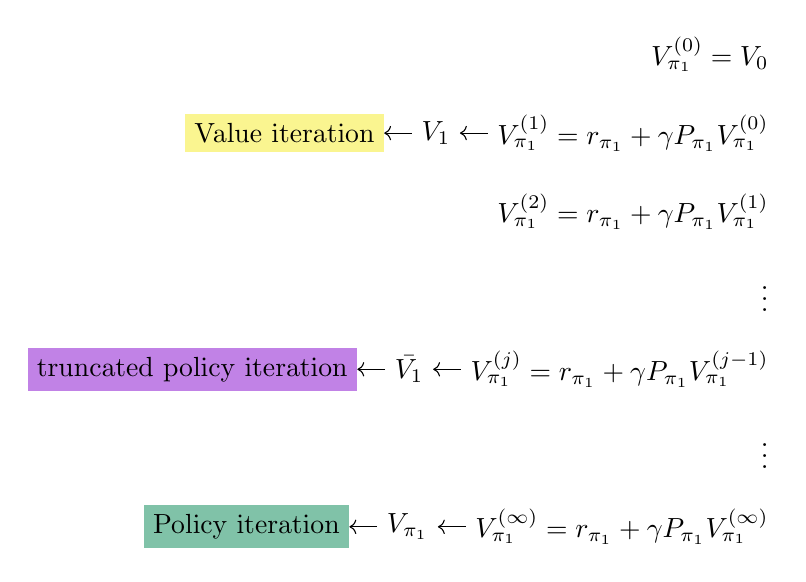
\begin{tikzpicture}
        \graph[grow left sep]{
            "$V_{\pi_1}^{(0)} = V_0$";
            "$V_{\pi_1}^{(1)}=r_{\pi_1}+\gamma P_{\pi_1}V_{\pi_1}^{(0)}$" -> "$V_1$" -> "Value iteration"[fill=myyellow!50];
            "$V_{\pi_1}^{(2)}=r_{\pi_1}+\gamma P_{\pi_1}V_{\pi_1}^{(1)}$";
            "$\vdots$";
            "$V_{\pi_1}^{(j)}=r_{\pi_1}+\gamma P_{\pi_1}V_{\pi_1}^{(j-1)}$" -> "$\bar{V_1}$" -> "truncated policy iteration"[fill=mypurple!50];
            "$ \!\vdots$ ";
            "$V_{\pi_1}^{(\infty)}=r_{\pi_1}+\gamma P_{\pi_1}V_{\pi_1}^{(\infty)}$" -> "$V_{\pi_1}$" -> "Policy iteration"[fill=mygreen!50];
        };    
    \end{tikzpicture}
\end{minipage}
and can have an observation from above process:
if we truncated policy iteration, for example, limit the maximum number of iteration, we can get a new algorithm which is a middle ground between two extremes. It is called \emph[myred]{Truncated Policy Iteration Algorithm}.\par
\begin{algorithm}[H]
    \caption{Truncated Policy Iteration algorithm}
    \KwIn The probability models $P(r|s,a)$ and $P(s'|s,a)$ for all (s,a) are known. Initial guess $\pi_0$.
    \KwOut The optimal State Value funtion and Policy.\\
    \While{$V_k \text{ (not } V_{\pi_k} \text{) }$ has not converged, for the kth iteration}{
        Select the initial value as $V_{k}^{(0)}=V_{k-1}$\\ 
        \tcc{truncate infinite j to a fixed number $j_{truncate}$}
        \While{$j < j_{truncate}$}{
            $V_{k}^{(j)} = \sum_a\pi(a|s)\sum_r\sum_{s'}\left[P(r|s,a)r+\gamma P(s'|s,a)V_k^{(j-1)}(s')\right]$
        } 
        Set $V_k =V_{k}^{j_{truncate}} $\\
        \tcc{Policy imporvement}
        \ForEach{state $s \in S$}{
            \ForEach{action $\in A(s)$}{
                $q_k(s,a) = \sum_rP(r|s,a)r + \gamma \sum_{s'}P(s'|s,a)V_k(s')$
            }
            $a_k^{*}(s)=\mathop{\arg \max}_{a}q_k(s,a)$ \\
            $\pi_{k+1}(a|s)=1 \text{ if } a=a_k^{*}\text{, else } \pi_{k+1}(a|s)=0$ \tcp{Policy updates}
        }
    }
\end{algorithm}

\section{Correctness of Algorithm}
Nomatter Value Iteration or Policy Iteration, iterative method(\ref{alg:vi}) for solving optimal Bellman Equation is the key point.The correctness of it is assured by \emph{Contract Mapping Theorem}. \par
\begin{definition}[Contract Mapping]
    The function $f(x)$ is a \emph[black]{contract mapping} if there exists $\gamma \in (0,1)$ such that 

    \begin{equation}
        \|f(x_1)-f(x_2)\| \le \gamma \|x_1-x_2\|
    \end{equation}
    for any $x_1,x_2 \in R^d$.
\end{definition}

\begin{theorem}[Contract mapping theorem]\label{thm:cm1}
    For any equation that has the form $x=f(x)$, where $x$ and $f(x)$ are real vectors, if$f$is a contract mapping, then the following properties hold:
    \begin{enumerate}
        \item Existence: there exists a fixed point $x^{*}$ satisfying $f(x^{*})=x^{*}$.
        \item Uniqueness: the fixed point is unique.
        \item Algorithm: the following iterative algorithm
                \begin{equation}
                    x_{k+1}=f(x_{k})
                \end{equation}
             where $(k=0,1,\cdots)$ will converge to $(x^{*})$ when $(k \to \infty)$
    \end{enumerate}
\end{theorem}

Before proving this theorem, we give the definition of \emph{fixed point} and \emph{Cauchy sequence}.
\begin{definition}[Fixed point]
    Consider a function $f(x)$, where $x \in R^{d}$ and $f: R^d \to R^d$. A point is  $x^{*}$ is a fixed point if  $f(x^*)=x^*$
\end{definition}

\begin{definition}[Cauchy sequence]
    A sequence $x_1,x_2,\cdots \in R$ is called \textbf{Cauchy Sequence} if for $\forall \epsilon >0$, there exists an integer N such that $\|x_m-x_n\|<\epsilon$, for all $m,n>N$. \par
    \emph{Cauchy Sequence is guaranteed to converge to a limit.}
\end{definition}

\begin{proof}
    \textbf{1. Convergent} \par
    For any $m>n$,
    \begin{align*}
        \|x_m-x_n\| &= \|x_m-x_{m-1}+x_{m-1}-x_{m-2}+x_{m-2}-\cdots +x_{n+1}-x_n\| \notag \\
        &\le \|x_m-x_{m-1}\| +\|x_{m-1}-x_{m-2}\| +\cdots +\|x_{n+1}-x_n\| \notag \\
    \end{align*}
    and $f$ is a contract mapping, we have
    \begin{align*}
        \|x_{k+1}-x_k\| &= \|f(x_k)-f(x_{k-1})\| \\
                        &\le \gamma \|x_k-x_{k-1}\| \\
                        &= \gamma \|f(x_{k-1})-f(x_{k-2})\| \\
                        &\le \gamma ^2 \|x_{k-1}-x_{k-2}\| \\
                        &\cdots \\
                        &\le \gamma ^k \|x_1-x_0\|
    \end{align*}

    So 
    \begin{align}
        \|x_m-x_n\| &\le \gamma ^{m-1}\|x_1-x_0\| + \gamma^{m-2}\|x_1-x_0\|+\cdots +\gamma^{n}\|x_1-x_0\| \notag \\
                    &= \frac{\gamma ^{n}(1-\gamma^{m-n})}{1-\gamma } \notag \\
                    &\le \frac{\gamma ^{n}}{1-\gamma }\|x_1-x_0\|
    \end{align}

    Now, for any $\epsilon>0$, we can always find an integer N such that $\|x_{m}-x_{n}\|<\epsilon$ for all $m,n>N$. So
    $\{x_{k+1}=f(x_k)\}_{k=0}^{\infty}$ is a \emph{Cauchy sequence} and hence converge to a limit point which is denoted as $x^*=\lim_{k\to \infty}x_k$ \newline

    \textbf{2. The limit point is a fixed point} \par
    Because
    \begin{equation*}
        \|f(x_k)-x_k\| = \|x_{k+1}-x_k\| \le \gamma ^k\|x_1-x_0\|
    \end{equation*}
    $\|f(x_{k})-x_{k}\|$ converges to zero exponentially. We get $f(x^{*})=x^*$ \newline

    \textbf{3. Uniqueness} \par
    Suppose there is another fixed point $x'$ which satisfies $f(x')=x'$, then
    \begin{equation}
        \|x'-x^*\|=\|f(x')-f(x^*)\|\le \gamma \|x'-x^*\| \quad \text{(definition of contract mapping)}
    \end{equation}
    Since $0<\gamma<1$, this inequality holds if and only if $\|x' -x^*\|=0$
\end{proof}

Contract mapping theorem tells us, if a mapping is a contract mapping, a Cauchy sequence ${x_k}_{k=0}^{\infty}$ can be generated by an iterative method($x_{k+1}=f(x_k)$) and its limit is the fixed point of that mapping. \par

Here we demonstrate the right-hand side of equation $V_{*}^{}(s)$ is a contract mapping. Firstly, we define $r_{\pi}(s)$ and $p_{\pi}(s'|s)$ based on eq.(\ref{vs1}). 

\begin{align*}
  r_{\pi}(s) &= \sum_{a}\pi(a|s)\sum_{r}rP(r|s,a) \\
  P_{\pi}(s'|s) &= \sum_{a}\pi(a|s)P(s'|s,a)
\end{align*}

Suppose that the states are indexed as $s_{i}$ with $i=1,2,\cdots,n$, for state $s_{i}$ in eq.(\ref{vs1})

\begin{equation*}
V_{\pi}(s_i)=r_{\pi}(s_i)+\gamma \sum_{s_j}p_{\pi}(s_j|s_i)V_{\pi}(s_j)
\end{equation*}

{\linespread{1.13}\selectfont
Let $V_{\pi}=[V_{\pi}(s_1),V_{\pi}(s_1),\cdots,V_{\pi}(s_n)]^T \in \mathbb{R}^n$,  $r_{\pi}=[r_{\pi}(s_1),r_{\pi}(s_1),\cdots,r_{\pi}(s_n)]^T \in \mathbb{R}^n$, and $P_{\pi} \in \mathbb{R}^{n \times n}$ with $[P_{\pi}]_{ij}=P_{\pi}(s_i|s_j)$ Then we get the matrix form of eq.(\ref{vs1}) \par}

\begin{equation*} 
    V_{\pi}=r_{\pi}+\gamma P_{\pi}V_{\pi}
\end{equation*} 

Here is an example with four states:

\begin{equation*}
    \underbrace{\begin{bmatrix}
        V_{\pi}(s_{1}) \\
        V_{\pi}(s_{2})  \\
        V_{\pi}(s_{3}) \\
        V_{\pi}(s_{4})
    \end{bmatrix}}_{V_{\pi}}=
    \underbrace{\begin{bmatrix}
        r_{\pi}(s_{1}) \\
        r_{\pi}(s_{2})  \\
        r_{\pi}(s_{3}) \\
        r_{\pi}(s_{4})
    \end{bmatrix}}_{r_{\pi}}+\gamma
    \underbrace{\begin{bmatrix}
        P_{\pi}(s_{1}|s_{1}) & P_{\pi}(s_{2}|s_{1}) & P_{\pi}(s_{3}|s_{1}) & P_{\pi}(s_{4}|s_{1}) \\
        P_{\pi}(s_{1}|s_{2}) & P_{\pi}(s_{2}|s_{2}) & P_{\pi}(s_{3}|s_{2}) & P_{\pi}(s_{4}|s_{2}) \\
        P_{\pi}(s_{1}|s_{3}) & P_{\pi}(s_{2}|s_{3}) & P_{\pi}(s_{3}|s_{3}) & P_{\pi}(s_{4}|s_{3}) \\
        P_{\pi}(s_{1}|s_{4}) & P_{\pi}(s_{2}|s_{4}) & P_{\pi}(s_{3}|s_{4}) & P_{\pi}(s_{4}|s_{4})
    \end{bmatrix}}_{P_{\pi}}
    \begin{bmatrix}
        V_{\pi}(s_{1}) \\
        V_{\pi}(s_{2})  \\
        V_{\pi}(s_{3}) \\
        V_{\pi}(s_{4})
    \end{bmatrix}
\end{equation*}

Since under different state we should have different optimal policy,  the value of policy $\pi$ is determined by the states. The matrix form of Bellman Optimality Equation is:

\begin{equation}\label{vsm1}
    V^*=\max_{\pi}\left(r_{\pi}+\gamma P_{\pi}V^*\right)
\end{equation}

Right now, we can see if taking right-hand side of eq.(\ref{vsm1}) as a funtion $f$, optimal value funciton ($V^*$) will be the fixed point of $f(V)$. That is why we will demostrate $f$ is a contract mapping. \par

Considering given any two vectors $V_1,V_2 \in \mathbb{R}^{n}$, and $\pi_{1}=\mathop{\arg\max}_{\pi}(r_{\pi}+\gamma P_{\pi}V_{1})$ and $\pi_{2}=\mathop{\arg\max}_{\pi}(r_{\pi}+\gamma P_{\pi}V_{2})$ (notice that police $\pi$ is determined by states and that is why the mapping taking only $V$ as its variable rather than $V$ and $\pi$). Then

\begin{align*} 
    f(V_{1})&=r_{\pi_{1}}+\gamma P_{\pi_{1}}V_{1} \ge r_{\pi_{2}}+\gamma P_{\pi_{2}}V_{1} \\ 
    f(V_{2})&=r_{\pi_{2}}+\gamma P_{\pi_{2}}V_{2} \ge r_{\pi_{1}}+\gamma P_{\pi_{1}}V_{2} 
\end{align*} 

where $\ge$ is an elementwise comparison. \par
As a result, 
 
\begin{align*}
    f(V_{1})-f(V_{2}) &\le r_{\pi_{1}}+\gamma P_{\pi_{1}}V_{1}-r_{\pi_{1}}+\gamma P_{\pi_{1}}V_{2} \\ 
                      &=\gamma P_{\pi_{1}}(V_{1}-V_{2})\\ \\ 
    f(V_{2})-f(V_{1}) &\le r_{\pi_{2}}+\gamma P_{\pi_{2}}V_{2}-r_{\pi_{2}}+\gamma P_{\pi_{2}}V_{1} \\
                      & =\gamma P_{\pi_{2}}(V_{2}-V_{1})  \\
\end{align*} 

Therefore, 

\begin{equation*} 
    \gamma P_{\pi_{2}}(V_{1}-V_{2})\le f(V_{1})-f(V_{2}) \le \gamma P_{\pi_{1}}(V_{1}-V_{2}) 
\end{equation*} 

Define $z\doteq\max(|\gamma P_{\pi_{1}}(V_{1}-V_{2})|, |\gamma P_{\pi_{2}}(V_{1}-V_{2})|)$ and use infinite norm ($\|\cdot\|_{\infty}\doteq\max_{i}|x_{i}|$), we get

\begin{equation*}
    \|f(V_{1})-f(V_{2})\|_{\infty}\le\|z\|_{\infty}
\end{equation*}

and
\begin{equation*}
    z_{i}=\max(\gamma|P_{\pi_{1}}[i](V_{1}-V_{2})|,\gamma|P_{\pi_{2}}[i](V_{1}-V_{2})|)
\end{equation*}
where $z_{i}$ is the ith element in $z$ and $P_{\pi_{1,2}}[i]$ is the ith row in matrix $P_{\pi_{1,2}}$ .
Because $P_{\pi_{1,2}}[i]$ is a vector with all non-negative elements and the sum of the elements are equal to 1,  it follows that

\begin{equation*}
    |P_{\pi_{1}}[i](V_{1}-V_{2})|=P_{\pi_{1}}[i]|(V_{1}-V_{2})|\le\|V_{1}-V_{2}\|_{\infty},
\end{equation*}

Similarly,
\begin{equation*}
    |P_{\pi_{2}}[i](V_{1}-V_{2})|=P_{\pi_{2}}[i]|(V_{1}-V_{2})|\le\|V_{1}-V_{2}\|_{\infty}.
\end{equation*}

So
\begin{equation*}
    \|z\|_{\infty}=\max_{i}|z_{i}|\le\gamma\|V_{1}-V_{2}\|_{\infty}
\end{equation*}

Finally we conclude that $f(V)$ is a contract mapping because
\begin{equation*}
    \|f(V_{1})-f(V_{2})\|_{\infty}\le\gamma\|V_{1}-V_{2}\|_{\infty}\le\|V_{1}-V_{2}\|_{\infty}
\end{equation*}

According to \nameref{thm:cm1}, we can easily get the theorem:
\begin{theorem}
    For the Bellman Optimality Equation $V=f(V)=\max_{\pi}(r_{\pi}+\gamma P_{\pi}V)$, there always exists a unique solution $V^*$, which can be iteratively solved by
    \begin{equation}
        V_{k+1}=\max_{\pi}(r_{\pi}+\gamma P_{\pi}V_{k})
    \end{equation}
    The value of $V_{k}$ is converged exponentially to $V^*$ as $k\to \infty$ given any initial state $V_{0}$
\end{theorem}

For the two algorithm Value Iteration and Policy Iteration, Value Iteration directly uses iterative method to solve BOE (Bellman Optimality Equation) whereas Policy Iteration just improve policy. So we can confirm that Value Iteration can get the optimal state value function and optimal policy\sn{Solving $\pi^*$ can be easily obtained by $\pi^*=\mathop{arg max}_\pi(r_{\pi}+\gamma P_{\pi}V^*)$ once optimal State value function is obtained.}, but for Policy Iteration, we need to prove that it eventually find an optimal policy and optimal state value funciton.

\begin{lemma}[Policy improvement]\label{lem:policy-improve}
    In the policy improvement step, $\pi_{k+1}$ is better than $\pi_{k}$. That is, if $\pi_{k+1}=\mathop{\arg\max}_{\pi}(r_{\pi}+\gamma P_{\pi}V_{\pi_{k}})$, then $V_{\pi_{k+1}} \ge V_{\pi_{k}}$. 
\end{lemma}

\begin{proof}
    Since $V_{\pi_{k+1}}$ and $V_{\pi_{k}}$ are state value function, they satisfy the Bellman Equation:
    \begin{align*}
        V_{\pi_{k+1}} & = r_{\pi_{k+1}} + \gamma P_{\pi_{k+1}}V_{\pi_{k+1}} \\
        V_{\pi_{k}} & = r_{\pi_{k}} + \gamma P_{\pi_{k}}V_{\pi_{k}}
    \end{align*}
    Because $\pi_{k+1}=\mathop{\arg\max}_{\pi}(r_{\pi}+\gamma P_{\pi}V_{\pi_{k}})$, we know that,
    \begin{equation*}
        r_{\pi_{k+1}} + \gamma P_{\pi_{k+1}}V_{\pi_{k}} \ge r_{\pi_{k}} + \gamma P_{\pi_{k}}V_{\pi_{k}}
    \end{equation*}
    It then follows that,
    \begin{align*}
        V_{\pi_{k}} - V_{\pi_{k+1}} & = \left(r_{\pi_{k}} + \gamma P_{\pi_{k}}V_{\pi_{k}}\right) - \left(r_{\pi_{k+1}}+\gamma P_{\pi_{k+1}}V_{\pi_{k+1}}\right) \\
                                    & \le \left(r_{\pi_{k+1}} + \gamma P_{\pi_{k+1}}V_{\pi_{k+1}}\right) - \left(r_{\pi_{k+1}}+\gamma P_{\pi_{k+1}}V_{\pi_{k}}\right) \\
                                    & = \gamma P_{\pi_{k+1}}(V_{\pi_{k}}-V_{\pi_{k+1}})
    \end{align*}
    Therefore,
    \begin{align*}
    V_{\pi_{k}} - V_{\pi_{k+1}} & \le \gamma ^2 P_{\pi_{k+1}}^2(V_{\pi_{k}}-V_{\pi_{k+1}}) \le \cdots \\
                                & \le \gamma ^n P_{\pi_{k+1}}^n(V_{\pi_{k}}-V_{\pi_{k+1}}) \\
                                &\le \lim_{ n \to \infty }\gamma ^n P_{\pi_{k+1}}^n(V_{\pi_{k}}-V_{\pi_{k+1}}) = 0 
    \end{align*}
    The limit is due to $\gamma<1$ and $P_{\pi_{k+1}}^n$ is a non-negative stochastic matrix for any $n$
\end{proof}

Before demonstrating that policy iteration alogorithm can get optimal value function, we recall converge of sequence. For monotonic sequence, its convergence can be guaranteed by theorem below:
\begin{theorem}[Convergence of monotonic sequences]\label{thm:cms}
    If the sequence $\{x_{k}\}$ is non-increasing and bounded from below:
    \begin{enumerate}
        \item Non-increasing: $x_{k+1} \le x_{k}$
        \item Similarly, if $\{x_{k}\}$ is non-decreasing and have a upper bound, then the sequence is convergent
    \end{enumerate}
    then $x_{k}$ converges to a value, which is the limit of $\{x_{k}\}$, as $k\to \infty$.
\end{theorem}
Similarly, if $\{x_{k}\}$ is non-decreasing and have a upper bound, then the sequence is convergent.

Considering the non-monotonic sequence, we also have a similiar converegence.

\begin{theorem}[Convergence of non-monotonic sequence]
    if the sequences is non-negative $x_{k}\ge 0$ and satisfies:
    \begin{equation}\label{nonmono-condition}
        \sum_{k=1}^{\infty}(x_{k+1}-x_{k})^+ < \infty
    \end{equation}

    then $\{x_{k}\}$ converges as $k \to \infty$. \\
    The definition of symbol $(\cdot)^+$ is:
    For any $z \in \mathbb{R}$, define

    \begin{equation*}
        z^+ \doteq
            \begin{cases}
                z & \text{if } z\ge 0, \\ 
                0 & \text{if } z<0. \\
            \end{cases}
    \end{equation*}

    Similarly, the definition of symbol $(\cdot)^-$ is:

    \begin{equation*}
        z^- \doteq
            \begin{cases}
                z & \text{if } z\le 0, \\ 
                0 & \text{if } z>0. \\
            \end{cases}
    \end{equation*}
\end{theorem}

\begin{proof}
    To analyze the convergence of non-monotonic sequences $\{x_{k}\}$, we can use symbols above to rewrite it as:

    \begin{align*}
        x_{k} &= x_{k} - x_{k-1} + x_{k-1} - x_{k-2}+\cdots + x_{2}-x_{1}+x_{1} \\
            &= \sum_{i=1}^{k-1}(x_{i+1}-x_{i})+x_{1} \\ 
            &\doteq S_{k} + x_{1}
    \end{align*}

    Note $S_{k}=\sum_{i=1}^{k-1}(x_{i+1}-x_{i})$ can be decomposed as:

    \begin{equation*}
        S_{k}=S_{k}^+ + S_{k}^-
    \end{equation*}
    where 
    \begin{align*}
        S_{k}^+ &= \sum_{i=1}^{k-1}(x_{i+1}-x_{i})\text{, for all } i \text{ which }x_{i+1}-x_{i} \ge 0 \\
        S_{k}^- &=\sum_{i=1}^{k-1}(x_{i+1}-x_{i})\text{, for all } i \text{ which }x_{i+1}-x_{i}<0
    \end{align*}

    Obviously, sequence $\{S_{k}^+\}$ is non-decreasing whereas $\{S_{k}^-\}$ is non-increasing. \\[6pt]
    Because $x_{k}\ge 0$, then $S_{k}^-\ge - S_{k}^+ - x_{1}$. So if $\{S_{k}^+\}$ has a upper bound, $\{S_{k}^-\}$ also has a lower bound, and vice versa. \\[6pt]
    Now the convergence of non-negative and non-monotonic sequences which satisfy the condition \ref{nonmono-condition} can be easily proved.
    First, the condition \ref{nonmono-condition} indicates that $\{S_{k}^+\}$ has a upper bound. Since $\{S_{k}^+\}$ is non-decreasing, the convergence of $\{S_{k}^+\}$ immediately follows from theorem 1. Suppose that $\{S_{k}^+\}$ converges to $S_{*}^+$. \\[6pt]
    Second, because $\{S_{k}^+\}$ has a upper bound, the non-increasing sequence $\{S_{k}^-\}$ also has a lower bound.  We also immediately get the convergence of $\{S_{k}^-\}$ based on theorem 1. Suppose that $\{S_{k}^-\}$ converges to $S_{*}^-$. \\[6pt]
    Finally, because $x_{k}=S_{k}^+ + S_{k}^- +x_{1}$, the convergence of $\{S_{k}^+\}$ and $\{S_{k}^-\}$ implies that $\{x_k\}$ converges to $x_{1}+S_{*}^++S_{*}^-$.
\end{proof}
In Policy iteration, we obtain two sequence, one is the sequence of policies:
\[
    \{\pi_{1},\pi_{2}, \cdots, \pi_{k}, \cdots\}
\]and the other is the sequence of state value function: 
\[
    \{V_{\pi_{1}},V_{\pi_{2}},\cdots,V_{\pi_{k}},\cdots\}.
\]Based on the Policy Improvement Lemma, we know that the sequence of state value function is a non-decreasing sequence and bounded by $V_{*}$ and it follows from \nameref{thm:cms} that $V_{\pi_{k}}$ converges to a constant value $V_{\infty}$, when $k \to \infty$. The final step is to demonstrate $V_{\infty}=V_{*}$\sn{Convergent value may not equal to bound!}.

\begin{remark}
    The idea of the proof is to show that the policy algorithm has a faster convergent speed than the value iteration. What the idea means is that as value iteration can converges to the optimal value sate $V_{*}$, with \emph[mypurple!80]{squeeze theorem}($V_{*}$ is the lower bound of the sequence of state value function which is generated by policy iteration algorithm since policy iteration has a faster convergent speed than value iteration and according to the definition, $V_{*}$ is the upper bound of the sequence), policy iteration is able to converge to $V_{*}$.
\end{remark}
Here is the proof,
\begin{proof}
    In particular, to prove the convergence of $\{V_{\pi_{k}}\}_{k=0}^{\infty}$, we introduce another sequence $\{V_{k}\}_{k=0}^{\infty}$ generated by
    \begin{equation}
    V_{k+1}=\max_{\pi_{k}}\left(r_{\pi_{k}}+\gamma P_{\pi_{k}}V_{k}\right)
    \end{equation}
    In fact, $\{V_{k}\}_{k=0}^{\infty}$ is exactly generated by value iteration. We use mathematical induction to demonstrate that the policy iteration can faster converge.
    \begin{enumerate}
        \item[1)] For $k=0$, we can always find a value $V_{0}$ that $V_{\pi_{0}} \ge V_{0}$ under any initial guess $\pi_{0}$
        \item[2)] Suppose that for $k\ge 0$, we have $V_{\pi_{k}}\ge V_{k}$
        \item[3)] For $k+1$, 
    \end{enumerate} 
    \begin{align*}
        V_{\pi_{k+1}}-V_{k+1} &= (r_{\pi_{k+1}}+\gamma P_{\pi_{k+1}}V_{\pi_{k+1}})-\max_{\pi_{k}}(r_{\pi_{k}}+\gamma P_{\pi_{k}}V_{k}) \\
                              &\ge (r_{\pi_{k+1}}+\gamma P_{\pi_{k+1}}V_{\pi_{k}})-\max_{\pi_{k}}(r_{\pi_{k}}+\gamma P_{\pi_{k}}V_{k}) \quad(Lemma\ \ref{lem:policy-improve}\ V_{\pi_{k+1}}\ge V_{\pi_{k}})\\
    \end{align*}

    Let $\pi'_{k}=\max_{\pi_{k}}(r_{\pi_{k}}+\gamma P_{\pi_{k}}V_{k})$. We should notice that in policy improvement step of both value and policy iteration, they travel throughout every state and every action. That means the candidate policy set for the optimal policy in the $kth$ iteration of policy iteration algorithm is as same as that in value iteration. \\[6pt]
    So if $\pi^*_{k}$ which is equal to $\pi_{k+1}$ (policy update step in Policy Iteration algorithm) is the optimal policy generated by the $kth$ iteration of policy iteration algorithm and $\pi'_{k}=\max_{\pi_{k}}(r_{\pi_{k}}+\gamma P_{\pi_{k}}V_{k})$ , we have $(r_{\pi_{k+1}}+\gamma P_{\pi_{k+1}}V_{\pi_{k}}) \ge (r_{\pi'_{k}}+\gamma P_{\pi'_{k}}V_{\pi_{k}})$ and,

    \begin{align*}
        V_{\pi_{k+1}}-V_{k+1} &\ge (r_{\pi'_{k}}+\gamma P_{\pi'_{k}}V_{\pi_{k}})-(r_{\pi'_{k}}+\gamma P_{\pi'_{k}}V_k) \\
                              &= \gamma P_{\pi'_{k}}(V_{\pi_{k}}-V_{k})
    \end{align*}

    Because $V_{\pi_{k}}\ge V_{k}$ and $P_{\pi'{k}}$ is non-negative, we have $V_{\pi_{k+1}}\ge V_{k+1}$. Therefore we can show by induction that $V_{k}\le V_{\pi_{k}}\le V^*$. Since $\{V_{k}\}_{k=0}^{\infty}$ converges to $V^*$, $V_{\pi_{k}}$ also converges to $V^*$.
\end{proof}

Now we have
\begin{theorem}[Convergence of Policy Iteration]
    The state value sequence $\{V_{\pi_{k}}\}_{k=0}^{\infty}$generated by Policy Iteration converges to the optimal state value $V_{*}$. As a result, the policy sequence $\{\pi_{k}\}_{k=0}^{\infty}$ converges to the optimal policy $\pi^{*}$
\end{theorem}



    \newpage
\end{document}
